\begin{exercise}
      {ID-a42903853dfdea65c0592ab2d4f701ca97723472}
      {Sieben Würfel}
  \ifproblem\problem
    Der abgebildete Körper besteht aus sieben gleich großen Würfeln und
    besitzt eine Oberfläche von 1\,920\,cm${}^{2}$. Wie groß ist sein Volumen?
    \begin{center}
      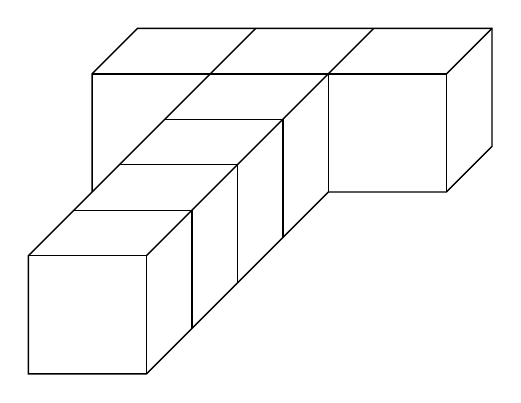
\begin{tikzpicture}[scale=1.5]
        % Umriss
        \draw [line width=0.5pt]
              ( 0, 1, 1) --
              ( 0, 1, 5) --
              ( 0, 0, 5) --
              ( 1, 0, 5) --
              ( 1, 0, 1) --
              ( 2, 0, 1) --
              ( 2, 0, 0) --
              ( 2, 1, 0) --
              (-1, 1, 0) --
              (-1, 1, 0) --
              (-1, 1, 1) --
              (-1, 0, 1);
        % vertikale und horizontale Kanten
        \draw [line width=0.5pt] ( 0, 1, 5) -- (1, 1, 5) -- (1, 0, 5);
        \draw [line width=0.5pt] ( 0, 1, 4) -- (1, 1, 4) -- (1, 0, 4);
        \draw [line width=0.5pt] ( 0, 1, 3) -- (1, 1, 3) -- (1, 0, 3);
        \draw [line width=0.5pt] ( 0, 1, 2) -- (1, 1, 2) -- (1, 0, 2);
        \draw [line width=0.5pt] ( 0, 1, 1) -- (1, 1, 1) -- (1, 0, 1);
        \draw [line width=0.5pt] ( 1, 1, 1) -- (2, 1, 1) -- (2, 0, 1);
        \draw [line width=0.5pt] (-1, 1, 1) -- (0, 1, 1);
        % diagonale Kanten
        \draw [line width=0.5pt] (1, 1, 5) -- (1, 1, 0);
        \draw [line width=0.5pt] (2, 1, 1) -- (2, 1, 0);
        \draw [line width=0.5pt] (0, 1, 1) -- (0, 1, 0);
      \end{tikzpicture}
    \end{center}
  \fi
  %\ifoutline\outline
  %\fi
  %\ifoutcome\outcome
  %\fi
\end{exercise}
